\documentclass[twoside]{book}

% Packages required by doxygen
\usepackage{fixltx2e}
\usepackage{calc}
\usepackage{doxygen}
\usepackage[export]{adjustbox} % also loads graphicx
\usepackage{graphicx}
\usepackage[utf8]{inputenc}
\usepackage{makeidx}
\usepackage{multicol}
\usepackage{multirow}
\PassOptionsToPackage{warn}{textcomp}
\usepackage{textcomp}
\usepackage[nointegrals]{wasysym}
\usepackage[table]{xcolor}

% Font selection
\usepackage[T1]{fontenc}
\usepackage[scaled=.90]{helvet}
\usepackage{courier}
\usepackage{amssymb}
\usepackage{sectsty}
\renewcommand{\familydefault}{\sfdefault}
\allsectionsfont{%
  \fontseries{bc}\selectfont%
  \color{darkgray}%
}
\renewcommand{\DoxyLabelFont}{%
  \fontseries{bc}\selectfont%
  \color{darkgray}%
}
\newcommand{\+}{\discretionary{\mbox{\scriptsize$\hookleftarrow$}}{}{}}

% Page & text layout
\usepackage{geometry}
\geometry{%
  a4paper,%
  top=2.5cm,%
  bottom=2.5cm,%
  left=2.5cm,%
  right=2.5cm%
}
\tolerance=750
\hfuzz=15pt
\hbadness=750
\setlength{\emergencystretch}{15pt}
\setlength{\parindent}{0cm}
\setlength{\parskip}{3ex plus 2ex minus 2ex}
\makeatletter
\renewcommand{\paragraph}{%
  \@startsection{paragraph}{4}{0ex}{-1.0ex}{1.0ex}{%
    \normalfont\normalsize\bfseries\SS@parafont%
  }%
}
\renewcommand{\subparagraph}{%
  \@startsection{subparagraph}{5}{0ex}{-1.0ex}{1.0ex}{%
    \normalfont\normalsize\bfseries\SS@subparafont%
  }%
}
\makeatother

% Headers & footers
\usepackage{fancyhdr}
\pagestyle{fancyplain}
\fancyhead[LE]{\fancyplain{}{\bfseries\thepage}}
\fancyhead[CE]{\fancyplain{}{}}
\fancyhead[RE]{\fancyplain{}{\bfseries\leftmark}}
\fancyhead[LO]{\fancyplain{}{\bfseries\rightmark}}
\fancyhead[CO]{\fancyplain{}{}}
\fancyhead[RO]{\fancyplain{}{\bfseries\thepage}}
\fancyfoot[LE]{\fancyplain{}{}}
\fancyfoot[CE]{\fancyplain{}{}}
\fancyfoot[RE]{\fancyplain{}{\bfseries\scriptsize Generated by Doxygen }}
\fancyfoot[LO]{\fancyplain{}{\bfseries\scriptsize Generated by Doxygen }}
\fancyfoot[CO]{\fancyplain{}{}}
\fancyfoot[RO]{\fancyplain{}{}}
\renewcommand{\footrulewidth}{0.4pt}
\renewcommand{\chaptermark}[1]{%
  \markboth{#1}{}%
}
\renewcommand{\sectionmark}[1]{%
  \markright{\thesection\ #1}%
}

% Indices & bibliography
\usepackage{natbib}
\usepackage[titles]{tocloft}
\setcounter{tocdepth}{3}
\setcounter{secnumdepth}{5}
\makeindex

% Hyperlinks (required, but should be loaded last)
\usepackage{ifpdf}
\ifpdf
  \usepackage[pdftex,pagebackref=true]{hyperref}
\else
  \usepackage[ps2pdf,pagebackref=true]{hyperref}
\fi
\hypersetup{%
  colorlinks=true,%
  linkcolor=blue,%
  citecolor=blue,%
  unicode%
}

% Custom commands
\newcommand{\clearemptydoublepage}{%
  \newpage{\pagestyle{empty}\cleardoublepage}%
}

\usepackage{caption}
\captionsetup{labelsep=space,justification=centering,font={bf},singlelinecheck=off,skip=4pt,position=top}

%===== C O N T E N T S =====

\begin{document}

% Titlepage & ToC
\hypersetup{pageanchor=false,
             bookmarksnumbered=true,
             pdfencoding=unicode
            }
\pagenumbering{alph}
\begin{titlepage}
\vspace*{7cm}
\begin{center}%
{\Large My Project }\\
\vspace*{1cm}
{\large Generated by Doxygen 1.8.15}\\
\end{center}
\end{titlepage}
\clearemptydoublepage
\pagenumbering{roman}
\tableofcontents
\clearemptydoublepage
\pagenumbering{arabic}
\hypersetup{pageanchor=true}

%--- Begin generated contents ---
\chapter{Namespace Index}
\section{Namespace List}
Here is a list of all namespaces with brief descriptions\+:\begin{DoxyCompactList}
\item\contentsline{section}{\mbox{\hyperlink{namespacecom}{com}} }{\pageref{namespacecom}}{}
\item\contentsline{section}{\mbox{\hyperlink{namespacecom_1_1hc}{com.\+hc}} }{\pageref{namespacecom_1_1hc}}{}
\item\contentsline{section}{\mbox{\hyperlink{namespacecom_1_1hc_1_1usb}{com.\+hc.\+usb}} }{\pageref{namespacecom_1_1hc_1_1usb}}{}
\end{DoxyCompactList}

\chapter{Hierarchical Index}
\section{Class Hierarchy}
This inheritance list is sorted roughly, but not completely, alphabetically\+:\begin{DoxyCompactList}
\item App\+Compat\+Activity\begin{DoxyCompactList}
\item \contentsline{section}{com.\+hc.\+usb.\+Main\+Activity}{\pageref{classcom_1_1hc_1_1usb_1_1_main_activity}}{}
\end{DoxyCompactList}
\end{DoxyCompactList}

\chapter{Class Index}
\section{Class List}
Here are the classes, structs, unions and interfaces with brief descriptions\+:\begin{DoxyCompactList}
\item\contentsline{section}{\mbox{\hyperlink{classcom_1_1hc_1_1usb_1_1_main_activity}{com.\+hc.\+usb.\+Main\+Activity}} }{\pageref{classcom_1_1hc_1_1usb_1_1_main_activity}}{}
\end{DoxyCompactList}

\chapter{File Index}
\section{File List}
Here is a list of all files with brief descriptions\+:\begin{DoxyCompactList}
\item\contentsline{section}{\mbox{\hyperlink{_main_activity_8java}{Main\+Activity.\+java}} }{\pageref{_main_activity_8java}}{}
\end{DoxyCompactList}

\chapter{Namespace Documentation}
\hypertarget{namespacecom}{}\section{Package com}
\label{namespacecom}\index{com@{com}}
\subsection*{Packages}
\begin{DoxyCompactItemize}
\item 
package \mbox{\hyperlink{namespacecom_1_1hc}{hc}}
\end{DoxyCompactItemize}

\hypertarget{namespacecom_1_1hc}{}\section{Package com.\+hc}
\label{namespacecom_1_1hc}\index{com.\+hc@{com.\+hc}}
\subsection*{Packages}
\begin{DoxyCompactItemize}
\item 
package \mbox{\hyperlink{namespacecom_1_1hc_1_1usb}{usb}}
\end{DoxyCompactItemize}

\hypertarget{namespacecom_1_1hc_1_1usb}{}\section{Package com.\+hc.\+usb}
\label{namespacecom_1_1hc_1_1usb}\index{com.\+hc.\+usb@{com.\+hc.\+usb}}
\subsection*{Classes}
\begin{DoxyCompactItemize}
\item 
class \mbox{\hyperlink{classcom_1_1hc_1_1usb_1_1_main_activity}{Main\+Activity}}
\end{DoxyCompactItemize}

\chapter{Class Documentation}
\hypertarget{classcom_1_1hc_1_1usb_1_1_main_activity}{}\section{com.\+hc.\+usb.\+Main\+Activity Class Reference}
\label{classcom_1_1hc_1_1usb_1_1_main_activity}\index{com.\+hc.\+usb.\+Main\+Activity@{com.\+hc.\+usb.\+Main\+Activity}}


Inheritance diagram for com.\+hc.\+usb.\+Main\+Activity\+:
\nopagebreak
\begin{figure}[H]
\begin{center}
\leavevmode
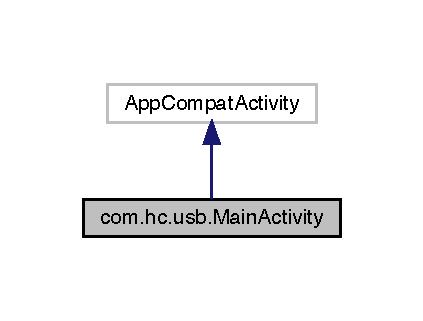
\includegraphics[width=203pt]{classcom_1_1hc_1_1usb_1_1_main_activity__inherit__graph}
\end{center}
\end{figure}


Collaboration diagram for com.\+hc.\+usb.\+Main\+Activity\+:
\nopagebreak
\begin{figure}[H]
\begin{center}
\leavevmode
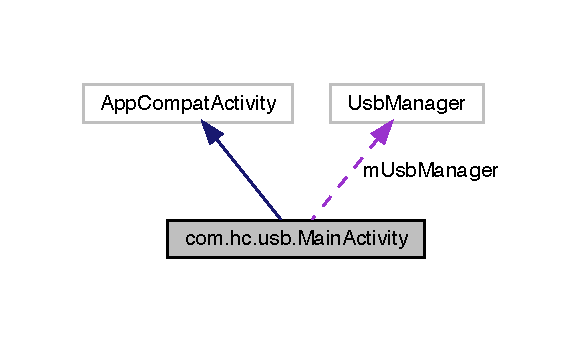
\includegraphics[width=280pt]{classcom_1_1hc_1_1usb_1_1_main_activity__coll__graph}
\end{center}
\end{figure}
\subsection*{Protected Member Functions}
\begin{DoxyCompactItemize}
\item 
void \mbox{\hyperlink{classcom_1_1hc_1_1usb_1_1_main_activity_acca2ed5d06d58ec04eb8380f568fa224}{on\+Create}} (Bundle saved\+Instance\+State)
\end{DoxyCompactItemize}
\subsection*{Private Member Functions}
\begin{DoxyCompactItemize}
\item 
void \mbox{\hyperlink{classcom_1_1hc_1_1usb_1_1_main_activity_abe05f9629f853d744ce45c776cf9930e}{print\+Usb\+Info}} ()
\end{DoxyCompactItemize}
\subsection*{Private Attributes}
\begin{DoxyCompactItemize}
\item 
Usb\+Manager \mbox{\hyperlink{classcom_1_1hc_1_1usb_1_1_main_activity_a34a5c06a51aa843f15b4c0677c48d288}{m\+Usb\+Manager}}
\end{DoxyCompactItemize}
\subsection*{Static Private Attributes}
\begin{DoxyCompactItemize}
\item 
static final String \mbox{\hyperlink{classcom_1_1hc_1_1usb_1_1_main_activity_a6ac2d8bf5d6fdb9288c6aae6a05eec3a}{T\+AG}} = \char`\"{}Main\+Activity\char`\"{}
\end{DoxyCompactItemize}


\subsection{Member Function Documentation}
\mbox{\Hypertarget{classcom_1_1hc_1_1usb_1_1_main_activity_acca2ed5d06d58ec04eb8380f568fa224}\label{classcom_1_1hc_1_1usb_1_1_main_activity_acca2ed5d06d58ec04eb8380f568fa224}} 
\index{com\+::hc\+::usb\+::\+Main\+Activity@{com\+::hc\+::usb\+::\+Main\+Activity}!on\+Create@{on\+Create}}
\index{on\+Create@{on\+Create}!com\+::hc\+::usb\+::\+Main\+Activity@{com\+::hc\+::usb\+::\+Main\+Activity}}
\subsubsection{\texorpdfstring{on\+Create()}{onCreate()}}
{\footnotesize\ttfamily void com.\+hc.\+usb.\+Main\+Activity.\+on\+Create (\begin{DoxyParamCaption}\item[{Bundle}]{saved\+Instance\+State }\end{DoxyParamCaption})\hspace{0.3cm}{\ttfamily [inline]}, {\ttfamily [protected]}}

Here is the call graph for this function\+:
\nopagebreak
\begin{figure}[H]
\begin{center}
\leavevmode
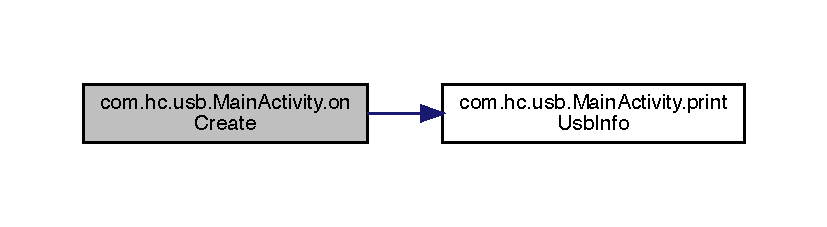
\includegraphics[width=350pt]{classcom_1_1hc_1_1usb_1_1_main_activity_acca2ed5d06d58ec04eb8380f568fa224_cgraph}
\end{center}
\end{figure}
\mbox{\Hypertarget{classcom_1_1hc_1_1usb_1_1_main_activity_abe05f9629f853d744ce45c776cf9930e}\label{classcom_1_1hc_1_1usb_1_1_main_activity_abe05f9629f853d744ce45c776cf9930e}} 
\index{com\+::hc\+::usb\+::\+Main\+Activity@{com\+::hc\+::usb\+::\+Main\+Activity}!print\+Usb\+Info@{print\+Usb\+Info}}
\index{print\+Usb\+Info@{print\+Usb\+Info}!com\+::hc\+::usb\+::\+Main\+Activity@{com\+::hc\+::usb\+::\+Main\+Activity}}
\subsubsection{\texorpdfstring{print\+Usb\+Info()}{printUsbInfo()}}
{\footnotesize\ttfamily void com.\+hc.\+usb.\+Main\+Activity.\+print\+Usb\+Info (\begin{DoxyParamCaption}{ }\end{DoxyParamCaption})\hspace{0.3cm}{\ttfamily [inline]}, {\ttfamily [private]}}



\subsection{Member Data Documentation}
\mbox{\Hypertarget{classcom_1_1hc_1_1usb_1_1_main_activity_a34a5c06a51aa843f15b4c0677c48d288}\label{classcom_1_1hc_1_1usb_1_1_main_activity_a34a5c06a51aa843f15b4c0677c48d288}} 
\index{com\+::hc\+::usb\+::\+Main\+Activity@{com\+::hc\+::usb\+::\+Main\+Activity}!m\+Usb\+Manager@{m\+Usb\+Manager}}
\index{m\+Usb\+Manager@{m\+Usb\+Manager}!com\+::hc\+::usb\+::\+Main\+Activity@{com\+::hc\+::usb\+::\+Main\+Activity}}
\subsubsection{\texorpdfstring{m\+Usb\+Manager}{mUsbManager}}
{\footnotesize\ttfamily Usb\+Manager com.\+hc.\+usb.\+Main\+Activity.\+m\+Usb\+Manager\hspace{0.3cm}{\ttfamily [private]}}

\mbox{\Hypertarget{classcom_1_1hc_1_1usb_1_1_main_activity_a6ac2d8bf5d6fdb9288c6aae6a05eec3a}\label{classcom_1_1hc_1_1usb_1_1_main_activity_a6ac2d8bf5d6fdb9288c6aae6a05eec3a}} 
\index{com\+::hc\+::usb\+::\+Main\+Activity@{com\+::hc\+::usb\+::\+Main\+Activity}!T\+AG@{T\+AG}}
\index{T\+AG@{T\+AG}!com\+::hc\+::usb\+::\+Main\+Activity@{com\+::hc\+::usb\+::\+Main\+Activity}}
\subsubsection{\texorpdfstring{T\+AG}{TAG}}
{\footnotesize\ttfamily final String com.\+hc.\+usb.\+Main\+Activity.\+T\+AG = \char`\"{}Main\+Activity\char`\"{}\hspace{0.3cm}{\ttfamily [static]}, {\ttfamily [private]}}



The documentation for this class was generated from the following file\+:\begin{DoxyCompactItemize}
\item 
\mbox{\hyperlink{_main_activity_8java}{Main\+Activity.\+java}}\end{DoxyCompactItemize}

\chapter{File Documentation}
\hypertarget{_main_activity_8java}{}\section{Main\+Activity.\+java File Reference}
\label{_main_activity_8java}\index{Main\+Activity.\+java@{Main\+Activity.\+java}}
\subsection*{Classes}
\begin{DoxyCompactItemize}
\item 
class \mbox{\hyperlink{classcom_1_1hc_1_1usb_1_1_main_activity}{com.\+hc.\+usb.\+Main\+Activity}}
\end{DoxyCompactItemize}
\subsection*{Packages}
\begin{DoxyCompactItemize}
\item 
package \mbox{\hyperlink{namespacecom_1_1hc_1_1usb}{com.\+hc.\+usb}}
\end{DoxyCompactItemize}

%--- End generated contents ---

% Index
\backmatter
\newpage
\phantomsection
\clearemptydoublepage
\addcontentsline{toc}{chapter}{Index}
\printindex

\end{document}
